\subsection{Data}

\plothere{franke function}

\begin{align}
    f(x, y) &= \frac{3}{4} \exp\left( -\frac{(9x - 2)^2}{4} - \frac{(9y - 2)^2}{4} \right) \nonumber \\
    &\quad + \frac{3}{4} \exp\left( -\frac{(9x + 1)^2}{49} - \frac{(9y + 1)^2}{10} \right) \nonumber \\
    &\quad + \frac{1}{2} \exp\left( -\frac{(9x - 7)^2}{4} - \frac{(9y - 3)^2}{4} \right) \nonumber \\
    &\quad - \frac{1}{5} \exp\left( -(9x - 4)^2 - (9y - 7)^2 \right)
\end{align}


\begin{figure}[h!]
\centering
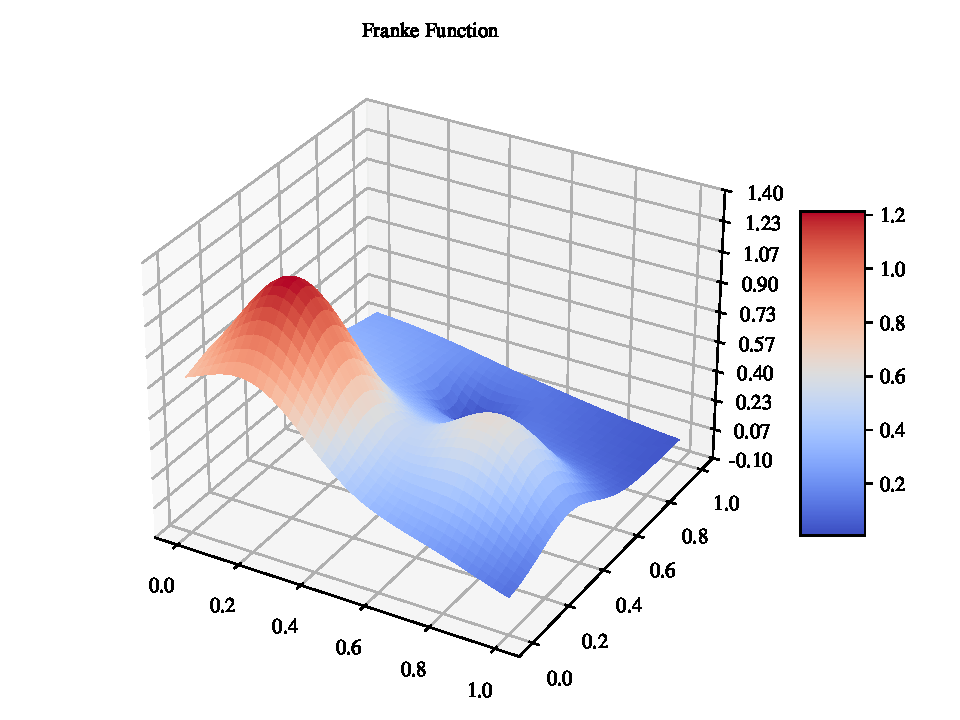
\includegraphics[width=1\linewidth]{project_1/figures/data/franke_func.pdf}
\caption{\mia{missing caption}}
\label{franke}
\end{figure}

\begin{figure}[h!]
\centering
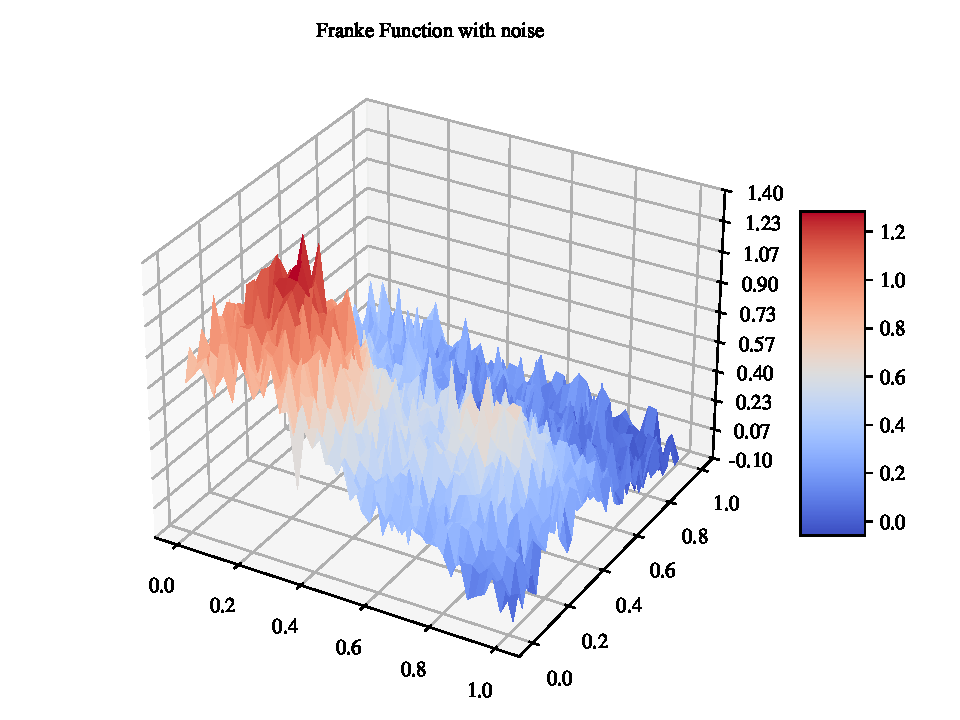
\includegraphics[width=1\linewidth]{project_1/figures/data/franke_func_noise.pdf}
\caption{\mia{missing caption}}
\label{franke_noise}
\end{figure}


\plothere{terrain data}
\gaute{Gaute must fill in}

\gaute{which scaler is used}
\gaute{grid search to find lambda}
\gaute{}